\documentclass{standalone}
\usepackage{tikz}
%\usetikzlibrary{...}
\begin{document}
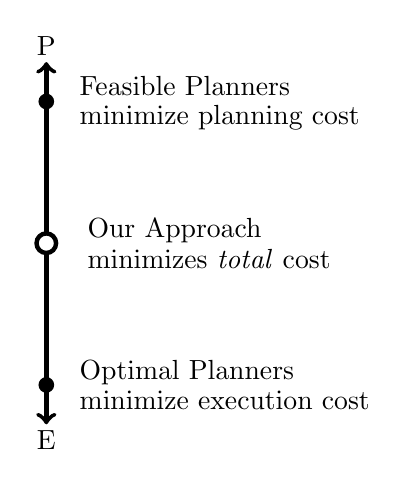
\begin{tikzpicture}
\draw[<->,ultra thick] (0,-2.3) -- (0,2.3);
\node at (0,2.5) {P};
\node at (0,-2.5) {E};
\node[circle,fill=black,inner sep=2] at (0,1.8) {};
\node[circle,fill=black,inner sep=2] at (0,-1.8) {};
\node[circle,draw,ultra thick,fill=white,inner sep=2.5] at (0,0) {};
\node[anchor=west] at (0.3,2.0) {Feasible Planners};
\node[anchor=west] at (0.3,1.6) {minimize planning cost};
\node[anchor=west] at (0.4, 0.16) {Our Approach};
\node[anchor=west] at (0.4,-0.2) {minimizes \emph{total} cost};
\node[anchor=west] at (0.3,-1.64) {Optimal Planners};
\node[anchor=west] at (0.3,-2.0) {minimize execution cost};
\end{tikzpicture}
\end{document}
